\chapter{COMPOSIÇÃO DA OBRA}

Dentre os componentes da instalação interativa aqui proposta, podemos destacar a interface, representada pelo sensor Microsoft Kinect, que parece invisível dado que o interator precisa apenas estar com o seu corpo presente no espaço para que a obra se materialize; o gerenciamento digital que é feito através de um computador e da utilização de Processing para execução e manutenção do programa; e, por fim, o dispositivo de saída de dados, aqui reprensentado por uma composição entre a malha de LEDs e o Arduino, traduzindo informação em luz.

Devido ao recurso de capturar objetos e movimentos no espaço, optou-se pelo uso do sensor Microsoft Kinect que, conectado a um computador, é responsável por captar a área onde os espectadores se encontram. Integrando-o a uma placa Arduino é possível controlar uma série de LEDs, dispostos em uma grade pendente ao teto. Cada LED possui cabos de fibra ótica \textit{side light} (com emissão de luz lateral) conectados à ele que se iluminam conforme os espectadores caminham sob a grade. Na figura \ref{fig:esquema} podemos ver um esquema de montagem da obra.

\begin{figure}[H]
    \centering
    \caption{Esquema de montagem da obra.}
	\vspace*{0,2cm}
    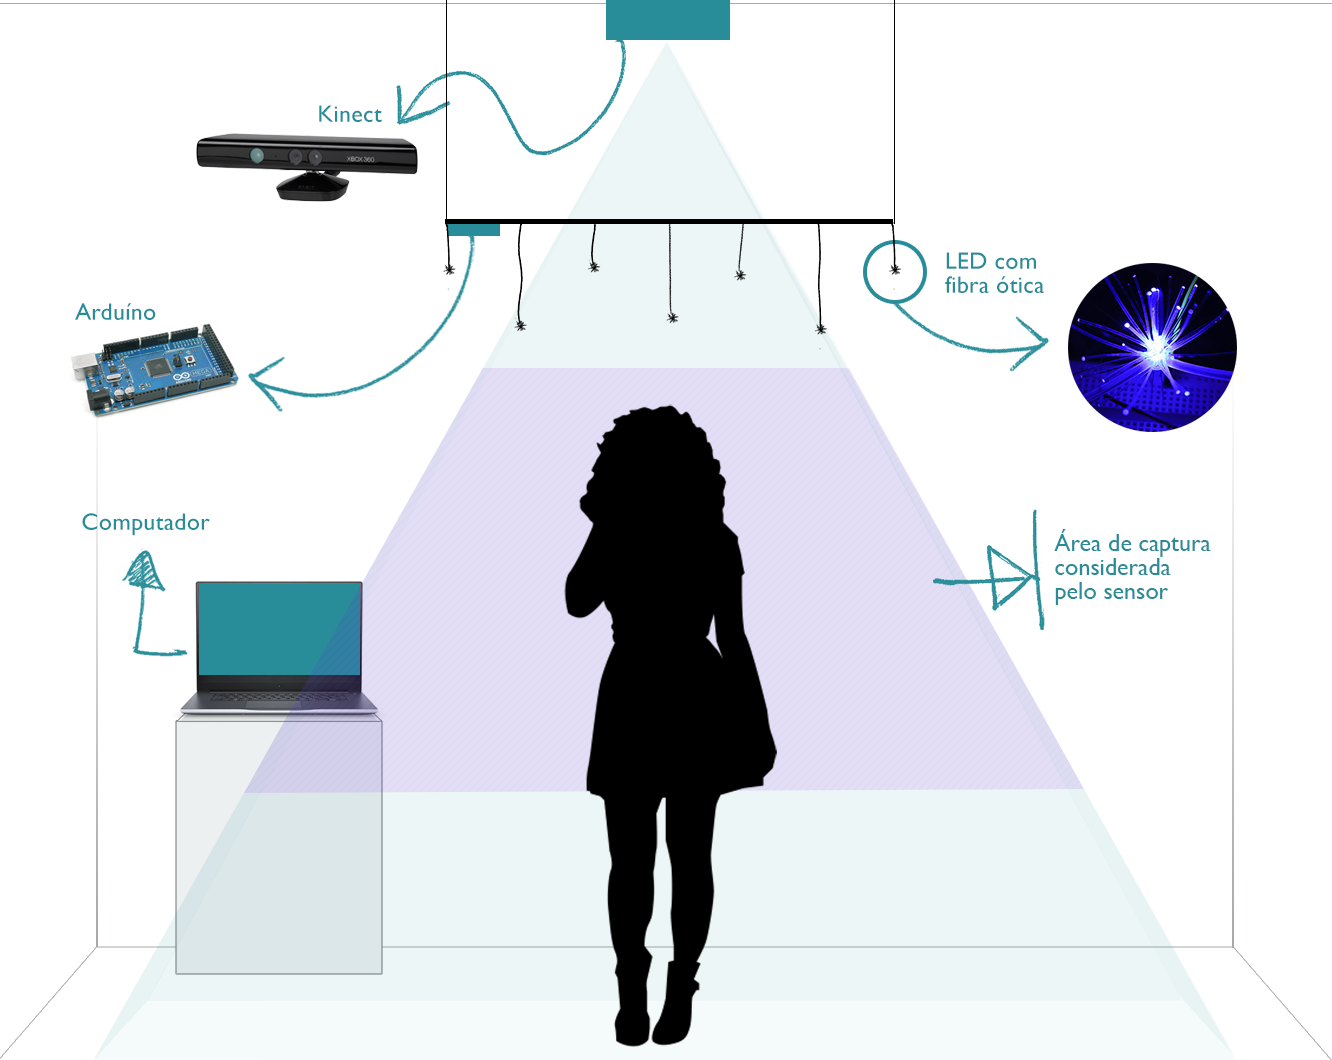
\includegraphics[width=0.8\textwidth]{./04-figuras/esquema}
    \label{fig:esquema}
\end{figure}
\vspace*{-0,9cm}
{\raggedright \fonte{Elaborada pela autora}}\\

Nas seções a seguir veremos um detalhamento dos componentes e nos aprofundaremos sobre o papel de cada um deles neste trabalho. 

\section{MICROSOFT KINECT}

O sensor Kinect é um dispositivo lançado em 4 de Novembro de 2010 como um acessório do console Xbox 360 da Microsoft. Orientado, principalmente, a indústria de jogos, foi criado para servir como uma forma de interação entre o utilizador e o console Xbox 360 através de gestos e comandos de voz. De acordo com a \citeonline{microsoft}, em sua primeira versão, é capaz de capturar imagens com 640x480 pixels a 30 fps. O aparelho é formado por um emissor e sensor de profundidade baseados em infravermelho, uma câmera RGB, um motor de inclinação e uma série de 4 microfones. Na figura \ref{fig:kinect_componentes} podemos ver a posição de cada um destes componentes no dispositivo.

\begin{figure}[H]
    \centering
    \caption{Componentes do sensor Kinect}
	\vspace*{0,2cm}
    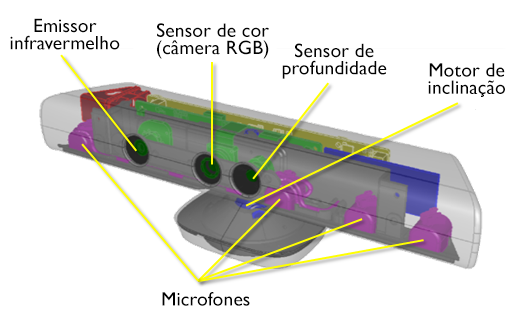
\includegraphics[width=0.8\textwidth]{./04-figuras/kinect_componentes}
    \label{fig:kinect_componentes}
\end{figure}
\vspace*{-0,9cm}
{\raggedright \fonte{Adaptado de \citeonline{microsoft}}}\\

Dentre seus componentes, o que mais nos interessa no contexto deste trabalho, é o sensor de profundidade. \citeonline{ashley} afirmam que a produção de dados tridimensionais é a principal função do Kinect. Ele difere de qualquer outro dispositivo de entrada justamente porque provê uma terceira dimensão e, para tanto, se utiliza de um emissor e uma câmera de infravermelho. Segundo \citeonline{lucero} o emissor de infravermelhos projeta um padrão estruturado de luz infravermelha, enquanto a câmera lê esses raios e interpreta a deformação da projeção, convertendo essa informação em valores de profundidade e, consequentemente, medindo a distância entre o objeto e o sensor. De acordo com \citeonline{correia} estas medidas baseiam-se em triangulação tendo em conta o emissor, a câmera e as posições dos pixels no cenário. A profundidade é codificada numa escala de cinzas. Quanto mais escuro o pixel, mais próximo do sensor está esse ponto no espaço. Sendo que, pixels pretos indicam que não existe informação de profundidade. Isto ocorre no caso dos pontos estarem muito longe, impossibilitando a sua captura, no caso de estarem numa área onde não haja pontos do emissor de infravermelhos, no caso de o objeto refletir mal a luz infravermelha ou, finalmente, no caso de os pontos estarem muito próximos do sensor, uma vez que o campo de visão do Kinect é limitado em cerca de 80 centímetros a 4 metros.

Considerando as limitações do Kinect, a que mais impactou este projeto é causada pela própria natureza da luz projetada pelo sensor. A luz emitida pelo projetor de infravermelho, ao se deparar com um objeto, gera uma sombra em outro que esteja numa distância maior. Segundo \citeonline{lucero} o resultado é que não se pode determinar a profundidade em zonas afetadas por estas sombras, pois elas criam zonas negras na imagem de profundidade, ou seja, pixels com valor zero, como pode ser visto na figura \ref{fig:kinect_sombras}. O impacto gerado aqui é devido à malha de LEDs se encontrar entre o Kinect e o espectador. A malha projeta uma sombra, criando pontos onde a área de intersecção entre o LED e o espectador pode não ser percebida. Para contornar este problema, ao invés de um ponto específico, adotou-se uma região maior que a espessura da sombra para garantir o acendimento dos LEDs.

\begin{figure}[H]
    \centering
    \caption{Efeito das sombras no sensor Kinect}
	\vspace*{0,2cm}
    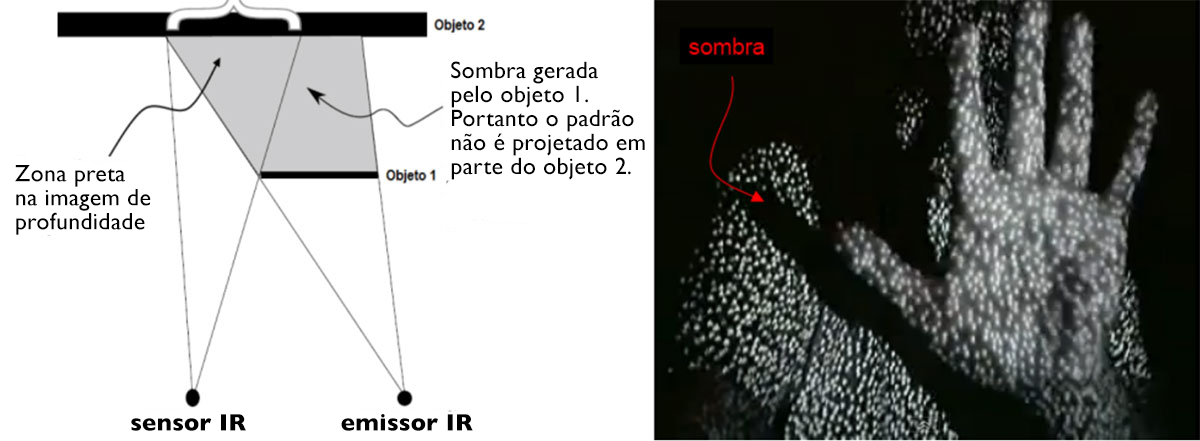
\includegraphics[width=0.8\textwidth]{./04-figuras/kinect_sombras}
    \label{fig:kinect_sombras}
\end{figure}
\vspace*{-0,9cm}
{\raggedright \fonte{Adaptado de \citeonline{lucero}}}\\

O Microsoft Kinect atua como interface da instalação interativa proposta neste trabalho sendo utilizado como fonte de entrada de dados (\textit{input}) para mapear o ambiente tridimensional. O mesmo foi configurado através do \textit{script} para considerar a captura de objetos em uma área específica entre a grade e o solo, dessa maneira, apesar de não ser possível impedir a criação de sombras, conforme falado anteriormente, podemos, pelo menos, desconsiderar a grade como uma fonte de entrada de dados. A figura \ref{fig:kinect_exemplo} mostra dois exemplos de imagens criadas a partir dos dados capturados pelo sensor. À esquerda temos um caso sem a configuração mencionada acima e à direita uma imagem com o sensor já calibrado.

\begin{figure}[H]
    \centering
    \caption{Imagens geradas a partir das informações capturadas pelo sensor Kinect.}
	\vspace*{0,2cm}
    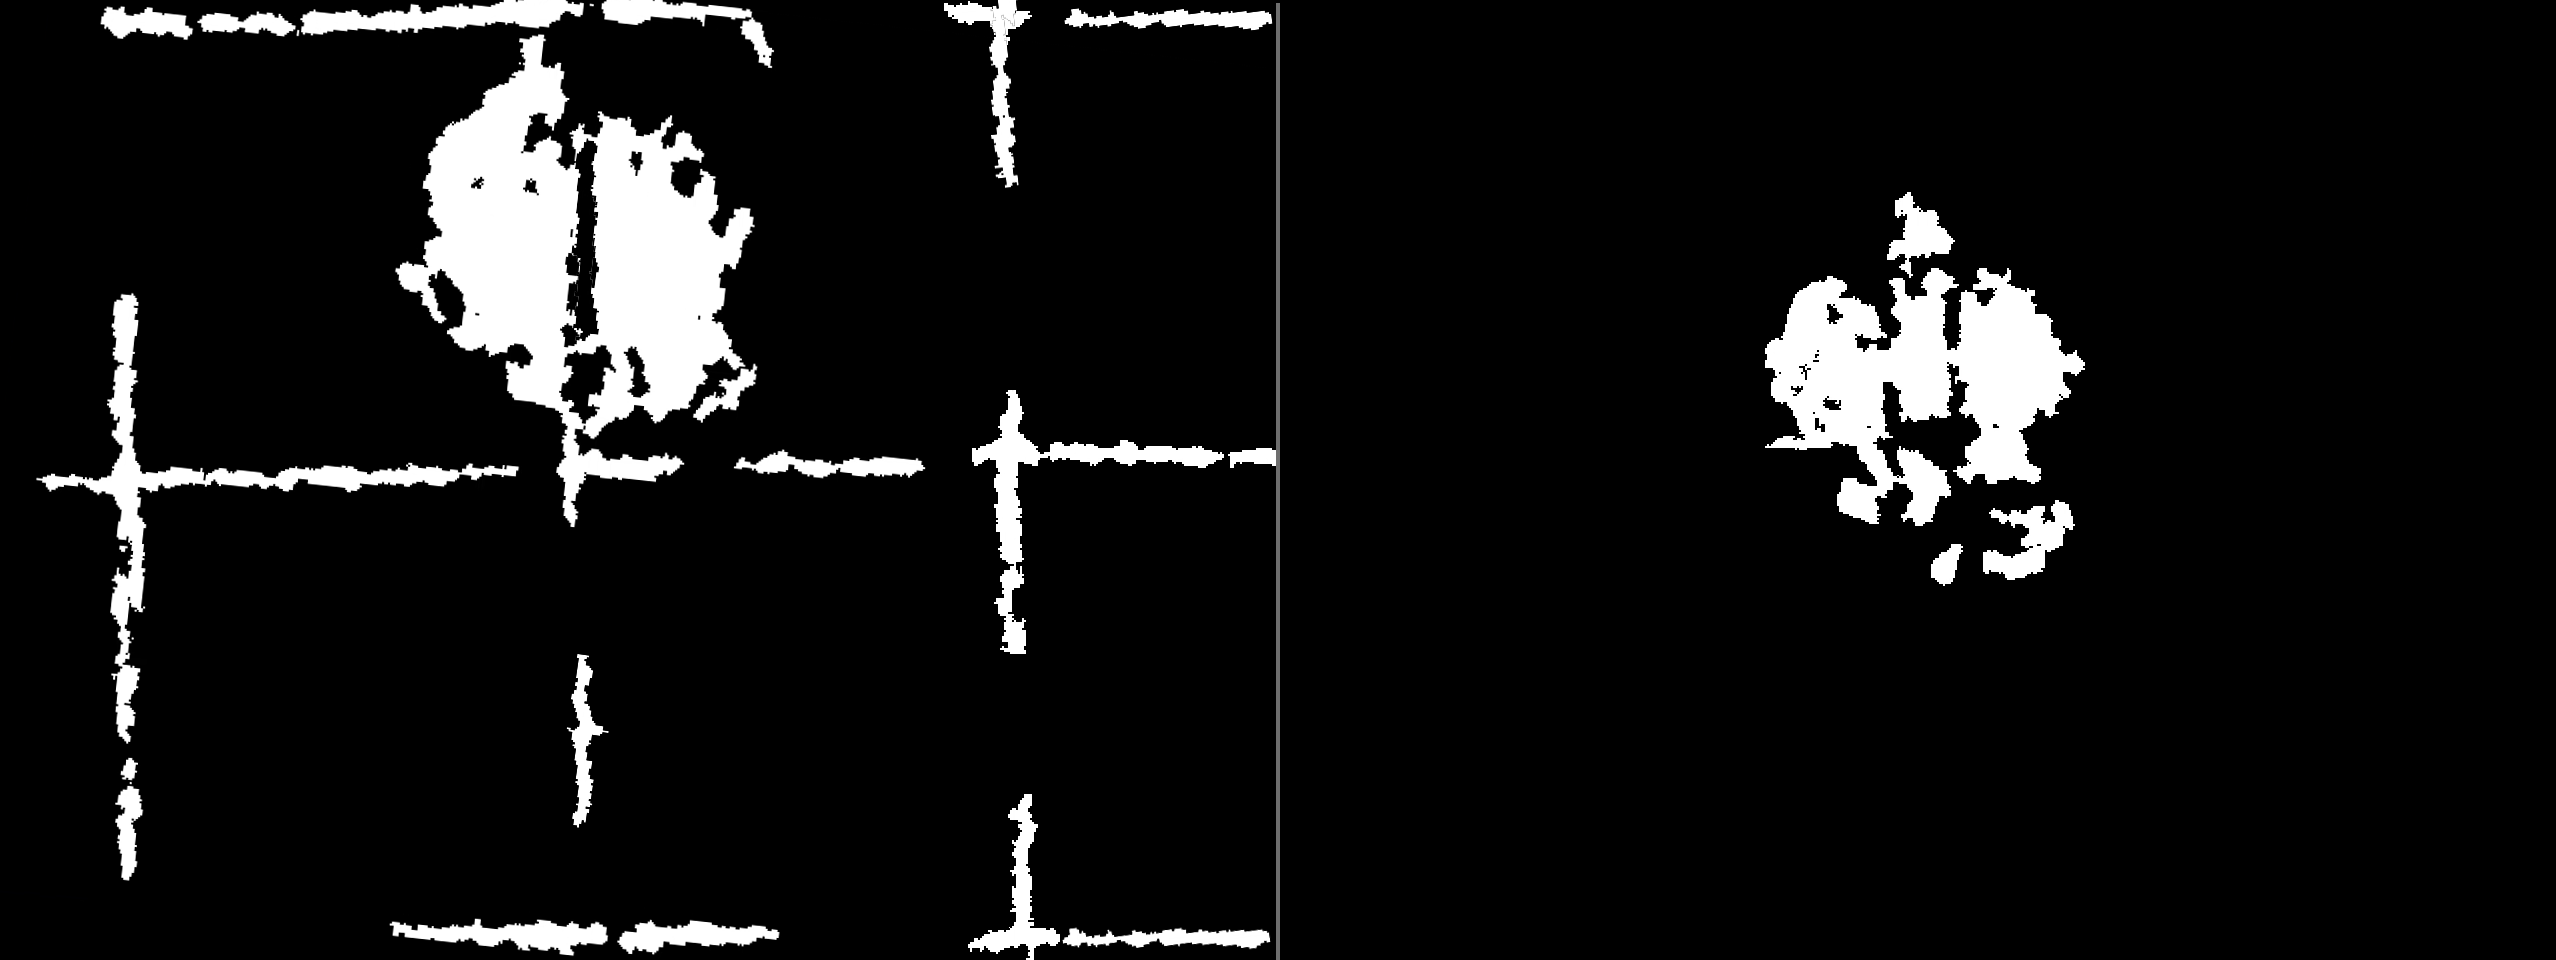
\includegraphics[width=0.8\textwidth]{./04-figuras/kinect_exemplo}
    \label{fig:kinect_exemplo}
\end{figure}
\vspace*{-0,9cm}
{\raggedright \fonte{Captura de tela gerada pelo sensor Kinect}}\\

Outro ponto importante sobre a figura acima é que as imagens possuem apenas \textit{pixels} pretos e brancos. Este comportamento foi programado de maneira intencional. Isto porque, no âmbito desta proposta, nos interessa saber se existe algo (ou alguém) na área em questão e não a distância que possa estar da grade de LEDs. Dessa forma, interatores de diferentes estaturas podem criar o mesmo efeito ao caminhar sob a malha, ainda que, pela diferente distancia do sensor, pessoas mais baixas pareçam menores na imagem capturada.


\section{PROCESSING}

De acordo com \citeonline[p. 115]{santos} Processing é a primeira ferramenta criada para artistas por artistas e o seu desenvolvimento foi iniciado no MIT Media Lab por dois estudantes de graduação: Casey Reas e Benjamin Fry. Segundo informações contidas no \textit{site} oficial do projeto, \citeonline{processing} é uma plataforma e uma linguagem de programação de código aberto (\textit{open source}) para prototipação de \textit{software} dentro do contexto das artes visuais. Disponível desde 2001, a Processing promoveu a alfabetização em \textit{software} dentro das artes visuais e a alfabetização visual dentro da tecnologia. Há dezenas de milhares de estudantes, artistas, designers, pesquisadores e amadores que usam Processing para aprender e criar protótipos.

O gerencimento digital da obra é realizado através de um computador que executa um programa escrito em Processing. Interpretando as informações fornecidas pelo Kinect, por meio da biblioteca \textit{Open Kinect for Processing} e, gerando uma imagem bidimensional, que é utilizada por um algorítimo de detecção de cor, é possível determinar quais LEDs devem permanecer apagados e quais devem acender na estrutura. A figura \ref{fig:script} nos dá uma ideia de como o programa foi construído. À esquerda temos uma imagem da câmera com pontos brancos e pretos desenhados sobre ela, onde, cada um deles representa um LED na estrutura física. À direita temos a imagem gerada a partir dos dados do sensor de profundidade, sendo que as áreas brancas identificam a presença do interator. As coordenadas e área dos pontos que visualizamos na imagem à esqueda foram utilizados para capturar fragmentos na imagem à direita. A cor predominante no fragmento de imagem (branco ou preto) determina a informação que é enviada ao Arduino para que este, por fim, acenda ou apague os LEDs. Pontos brancos identificam os LEDs acesos, enquanto os pretos identificam os apagados.


\begin{figure}[H]
    \centering
    \caption{Captura da camera e imagem gerada a partir do sensor de profundidade do Microsoft Kinect associadas à pontos que identificam os LEDs na estrutura física}
	\vspace*{0,2cm}
    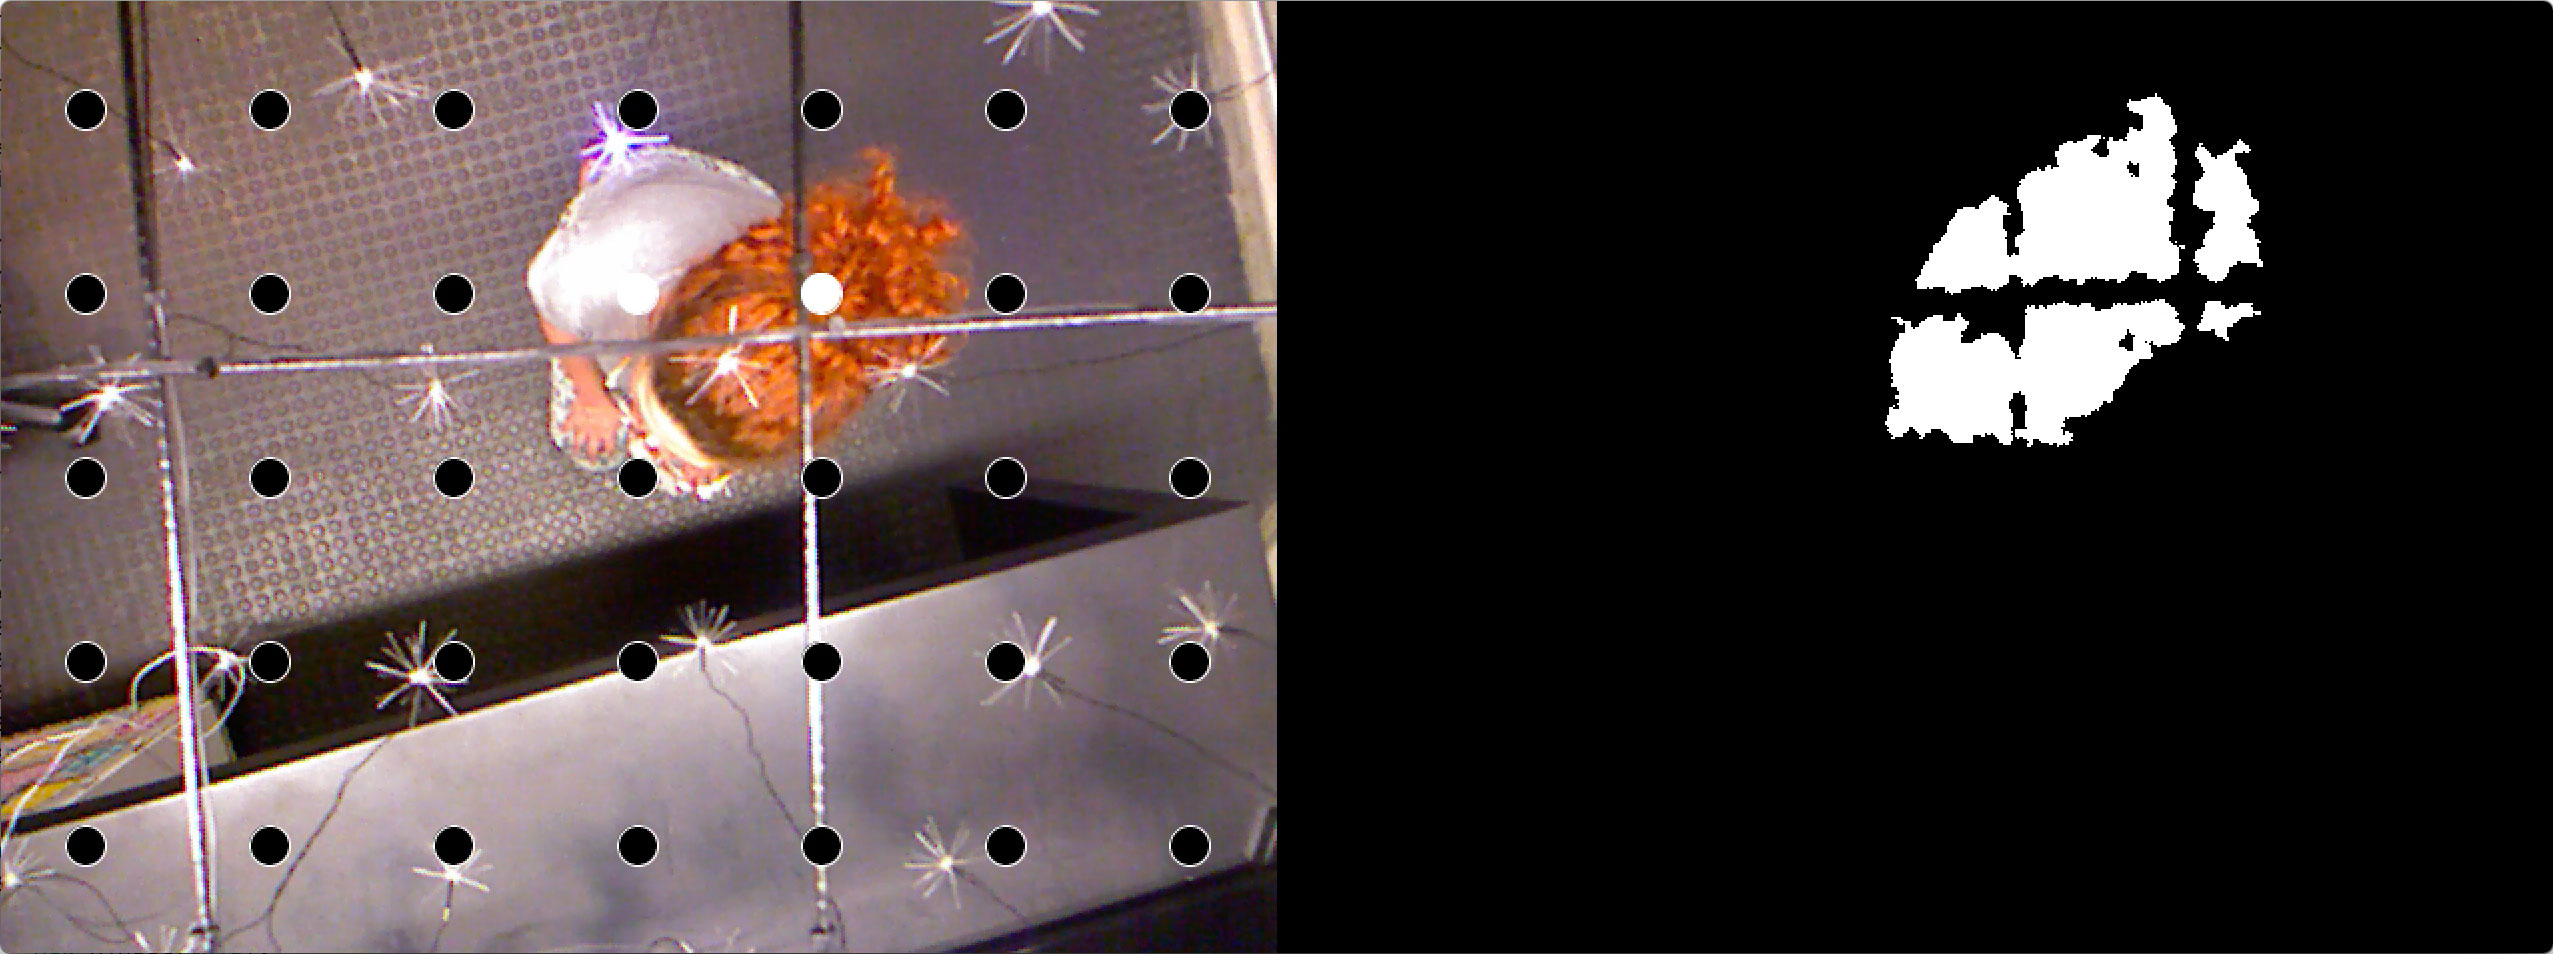
\includegraphics[width=0.8\textwidth]{./04-figuras/script}
    \label{fig:script}
\end{figure}
\vspace*{-0,9cm}
{\raggedright \fonte{Elaborada pela autora}}\\


\section{ARDUINO}

Para compreender o que é e para que serve o Arduino, podemos analisar a descrição presente no \textit{site} oficial do projeto:

\begin{citacao}
Arduino é uma plataforma de prototipagem eletrônica de \textit{hardware} livre e de placa única. O objetivo do projeto é criar ferramentas que são acessíveis, com baixo custo, flexíveis e fáceis de usar. Placas arduino são capazes de ler uma entrada como a luz em um sensor, um dedo pressionando um botão ou uma mensagem do Twitter e transformá-la em uma saída como ativar um motor, ligar um LED ou publicar alguma coisa na internet, por exemplo. É possível dizer à placa o que fazer enviando uma série de instruções ao microcontrolador. Para isso é necessário utilizar a linguagem de programação do Arduino (baseada em Wiring) e o seu \textit{software} (IDE - \textit{Integrated Development Environment} ou Ambiente de Desenvolvimento Integrado), baseada em Processing \cite{arduino}. 
\end{citacao}

Neste trabalho o Arduino foi utilizado para controlar a malha de LEDs (saída ou \textit{output}) recebendo as informações mapeadas pelo sensor Kinect (entrada ou \textit{input}). Cada LED é controlado individualmente, para isso, optou-se pela utilização do Arduino Mega 2560 (figura \ref{fig:arduino}) que possui 54 entradas/saídas digitais, suficientes para atender a proposta apresentada aqui sem adicionar complexidade ao circuito.

\begin{figure}[H]
    \centering
    \caption{Arduino Mega 2560}
	\vspace*{0,2cm}
    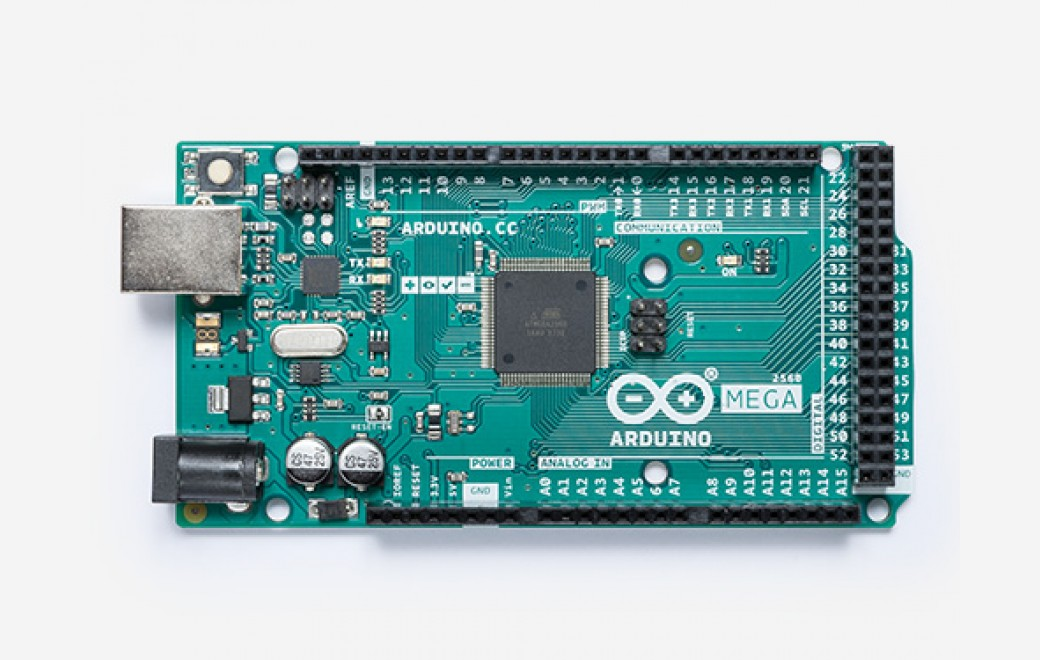
\includegraphics[width=0.8\textwidth]{./04-figuras/arduino}
    \label{fig:arduino}
\end{figure}
\vspace*{-0,9cm}
{\raggedright \fonte{\citeonline{arduino}}}\\

As pernas negativas dos LED foram soldadas em um fio conectado na porta \textit{ground} do Arduino, enquanto as pernas positivas foram conectadas à fios e plugadas individualmente em portas digitais. Na figura \ref{fig:breadboard} podemos ver o esquema equivalente a uma linha da matriz de LEDs. As demais são conectadas da mesma maneira e só não foram adicionadas para não poluir a imagem.

\begin{figure}[H]
    \centering
    \caption{Circuito de uma linha da matriz}
	\vspace*{0,2cm}
    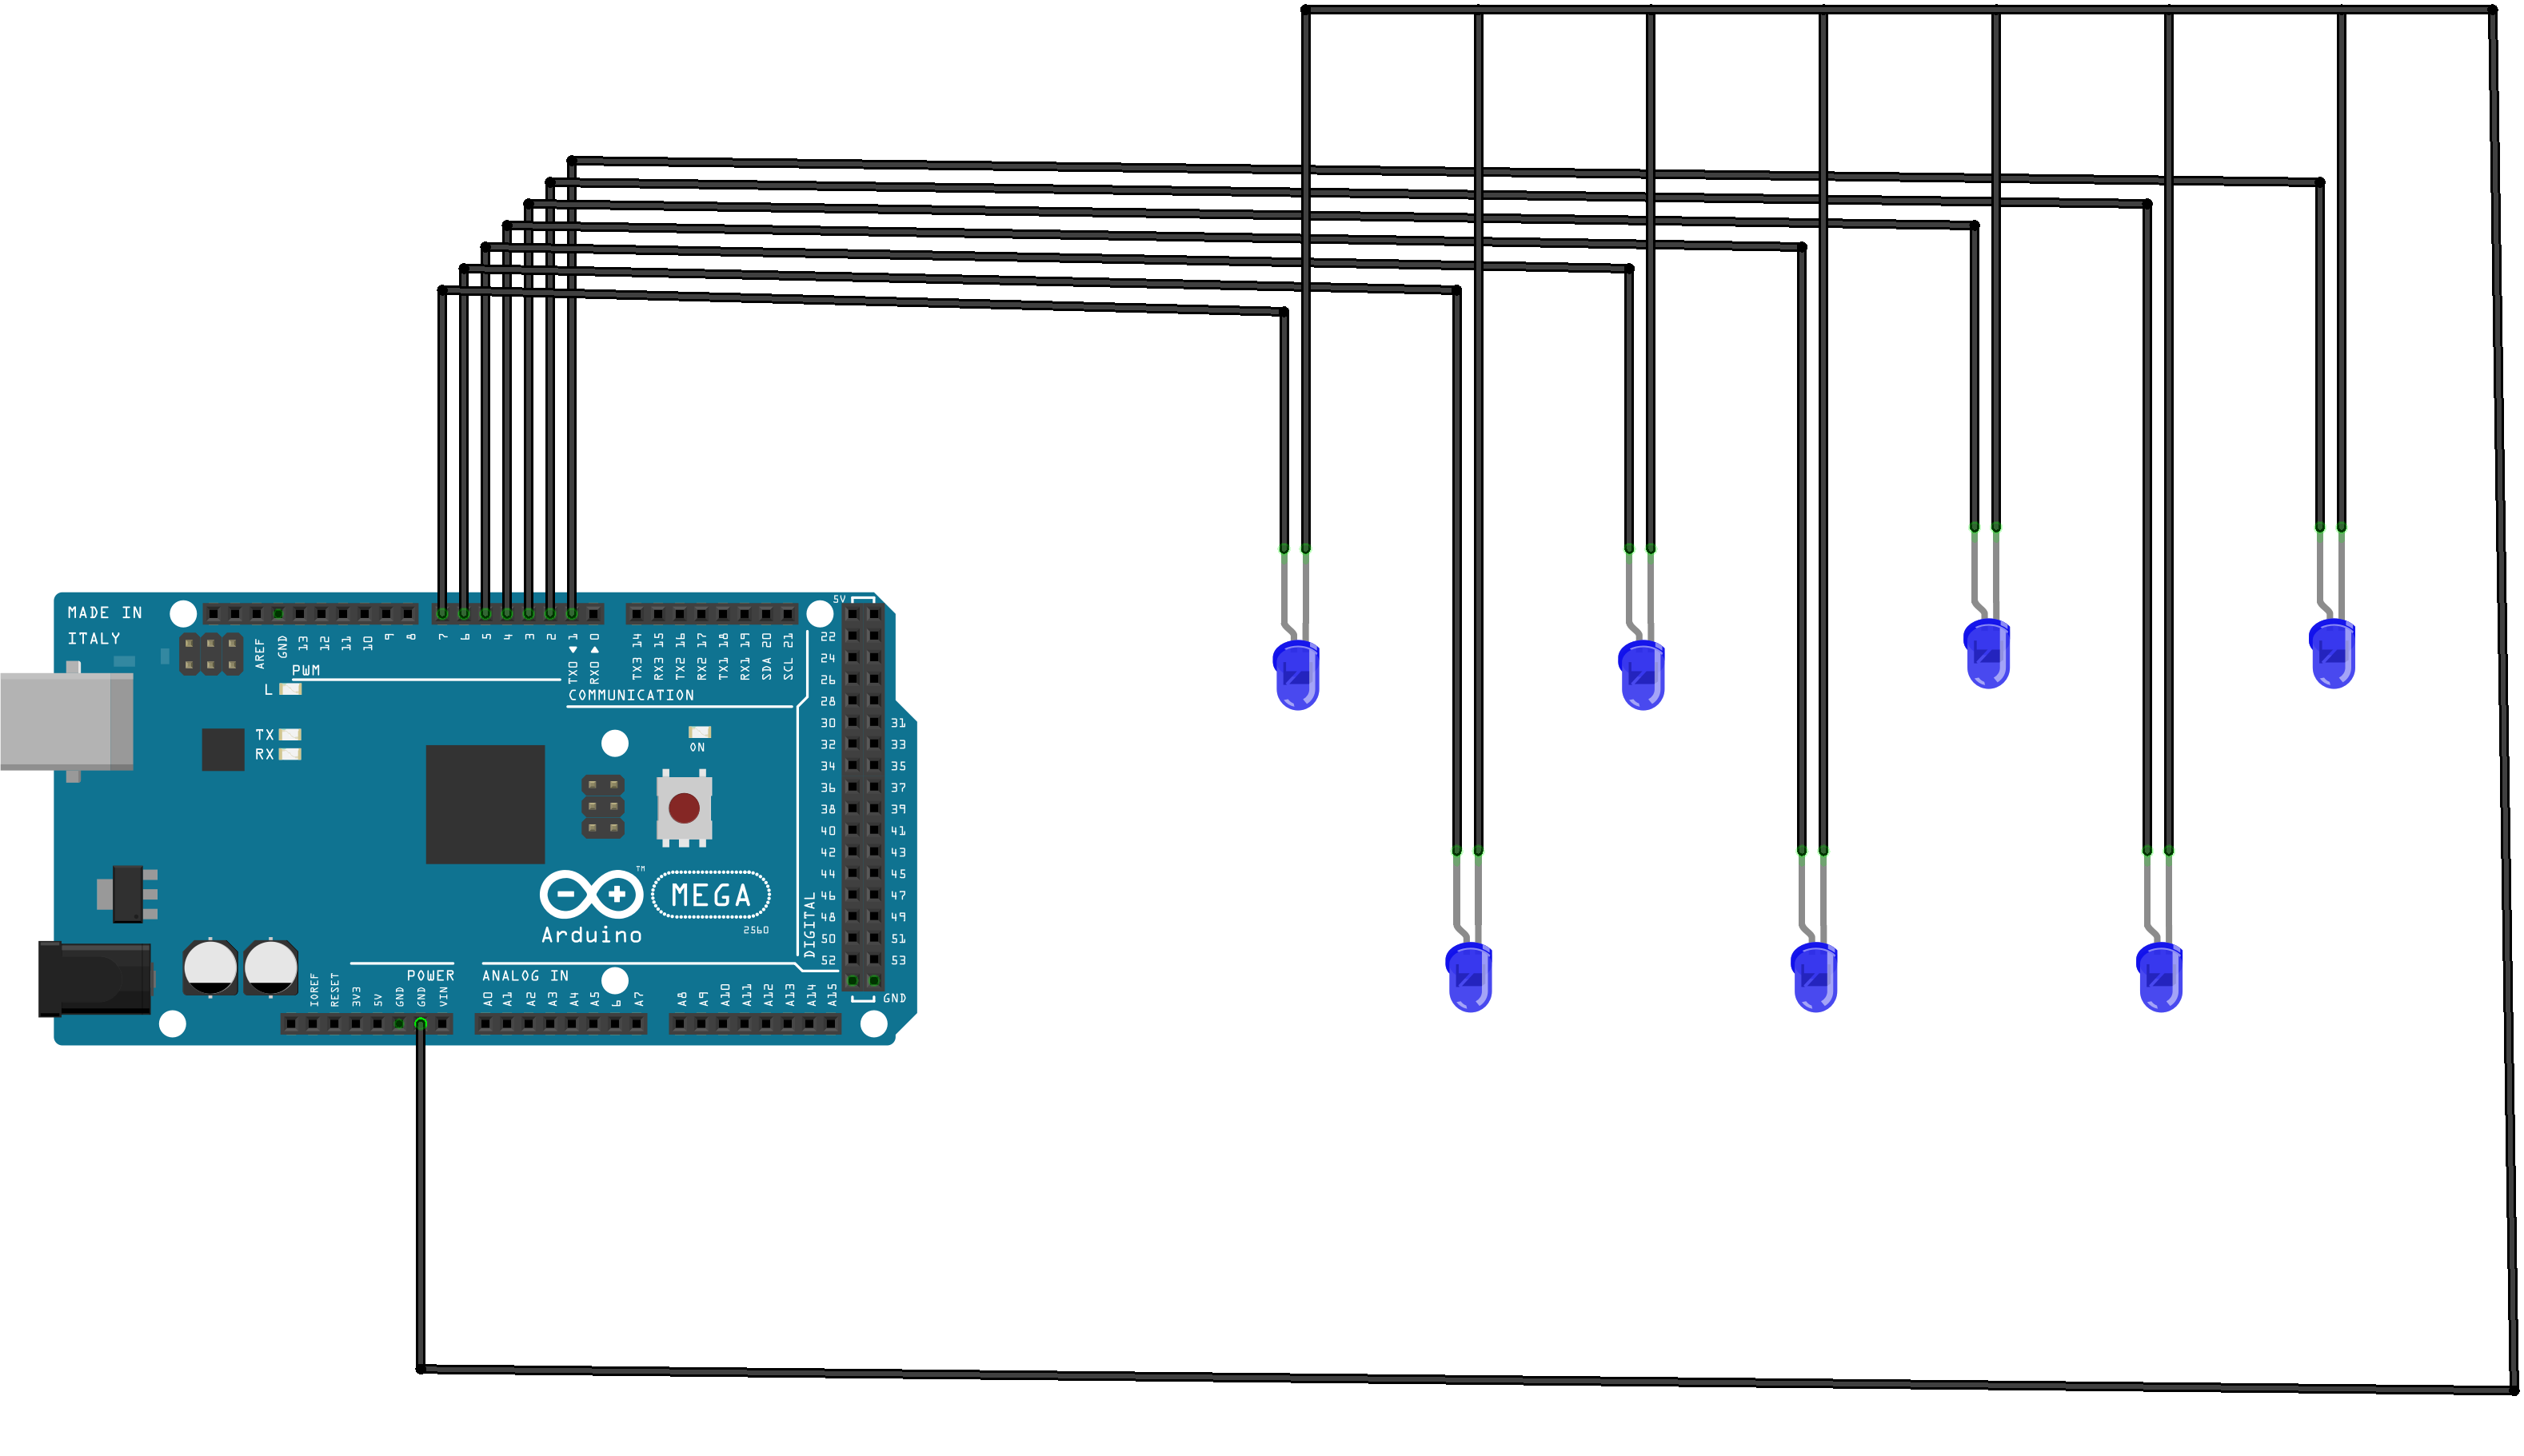
\includegraphics[width=0.8\textwidth]{./04-figuras/breadboard}
    \label{fig:breadboard}
\end{figure}
\vspace*{-0,9cm}
{\raggedright \fonte{Elaborada pela autora}}\\


Ainda no que se refere a hardware, \textit{hardware} foi constatada a necessidade de isolamento elétrico e de construir \textit{jumpers} plugáveis na placa. Por isso, a construção de cada elemento luminescente exigiu a utilização de alguns materiais. São eles:

\begin{itemize}
  \item 01 LED Alto Brilho Azul de 5 mm;
  \item 03 peças de tubo termo retrátil com 1 mm de espessura e 5 cm de comprimento para isolar as pernas do LED e a solda realizada junto ao fio negativo;
  \item 01 pino metálico macho para ligar a ponta do fio positivo no Arduino;
  \item 01 \textit{case} plástico para isolar o pino mencionado acima;  
  \item 02 pinos metálicos fêmea para conectar as pernas do LED ao fio;
  \item 40 cm de fibra ótica \textit{side light} com 0.5 mm de espessura cortada em pedaços de aproximadamente 3 cm;
  \item 40 cm de fibra ótica \textit{side light} com 0.75 mm de espessura cortada em pedaços de aproximadamente 3 cm;
  \item 20 cm de fibra ótica \textit{side light} com 1 mm de espessura cortada em pedaços de aproximadamente 3 cm;
  \item Fio AWG 30 de tamanho variado.
\end{itemize}


Já em relação à \textit{software} específico para o Arduino pouca coisa foi necessária. A biblioteca Firmata foi utilizada para servir como ponte de comunicação entre o Arduino e o computador. Através de um programa fornecido pela mesma e enviado para o microcontrolador, foi possível gerenciar a partir da Processing todos os recursos disponíveis na placa.

\section{MALHA DE LEDS}
\label{sec:malha}

A malha é composta primariamente por uma grade de 120 x 80 centímetros que delimita o espaço da instalação onde o espectador pode interagir com a obra. Como podemos ver na figura \ref{fig:malha}, esta grade possui intersecções a cada 20 centímetros, formando uma matriz de 5 linhas por 7 colunas. Cada intersecção possui um LED preso à ela, somando um total de 35 LEDs dispostos na obra.

\begin{figure}[H]
    \centering
    \caption{Esquema da malha de LEDs}
	\vspace*{0,2cm}
    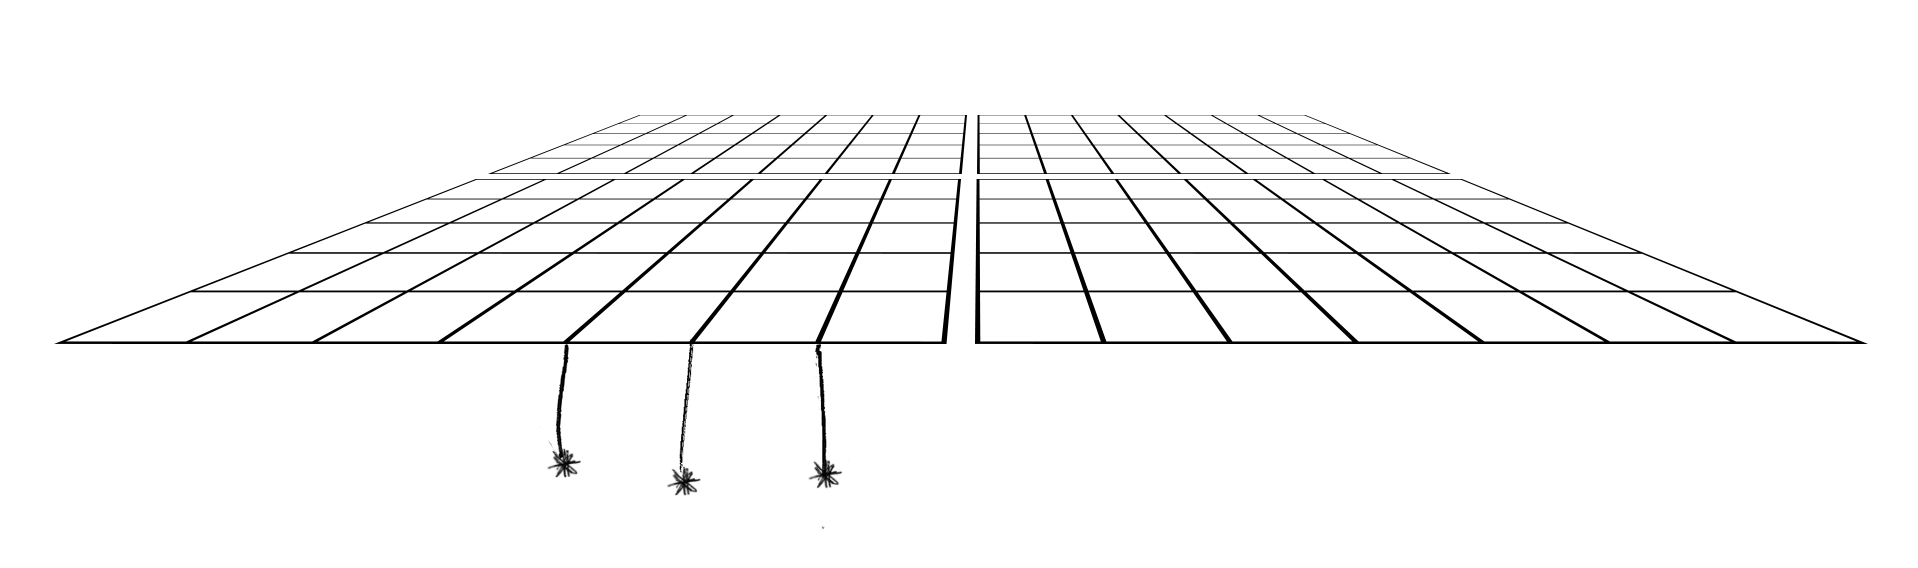
\includegraphics[width=0.8\textwidth]{./04-figuras/malha}
    \label{fig:malha}
\end{figure}
\vspace*{-0,9cm}
{\raggedright \fonte{Elaborada pela autora}}\\

Cada LED ocupa uma área na imagem processada pelo sistema computacional e conta com fios de fibra ótica, com emissão de luz lateral, de várias espessuras colados em sua extremidade. Quando o LED acende, a partir da interação com o usuário, a luz é transmitida pela fibra ótica, gerando vários pontos iluminados. Na figura \ref{fig:led_fibra_otica} podemos ver o exemplo de um desses LEDs, sendo que, no primeiro quadro o LED é exibido apagado, no segundo aceso em ambiente com alta luminosidade e, por fim, no terceiro quadro, aceso em ambiente com baixa luminosidade. 

\begin{figure}[H]
    \centering
    \caption{LED com fibra ótica em diferentes condições de luminosidade}
	\vspace*{0,2cm}
    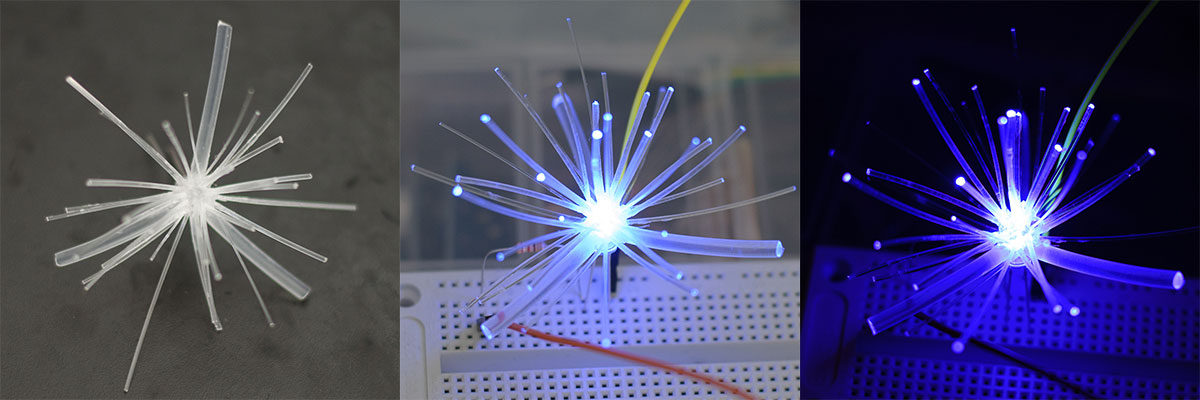
\includegraphics[width=0.8\textwidth]{./04-figuras/led_fibra_otica}
    \label{fig:led_fibra_otica}
\end{figure}
\vspace*{-0,9cm}
{\raggedright \fonte{Elaborada pela autora}}\\

A partir da imagem acima é possível constatar a diferença de exposição em ambientes com distintos graus de luminosidade. Ainda que a luz seja visível ao se observar o LED em um ambiente com alta incidência de luz e, isso viabilize a exposição do trabalho mesmo em condições como esta, se nota uma discrepância considerável quando voltamos nossos olhos para o terceiro quadrante, onde o LED é apresentado em ambiente com baixa luminosidade. A peça ganha destaque e a cor azul se propaga com maior intensidade, o que reforça a escolha do cubo preto como sendo o meio ideal para exibição desse trabalho.

\section{PROTÓTIPO}

Para validar o projeto foi construído um protótipo com o Microsoft Kinect, um computador, um Arduino Uno e 5 LEDs conectados à ele conforme pode ser visto na figura \ref{fig:prototipo}. Através da utilização de duas bibliotecas, \textit{Open Kinect for Processing} e Firmata, construiu-se um \textit{script} simplificado que controlava os dispositivos de entrada e saída de forma integrada, causando, assim, o acender e apagar dos LEDs de acordo com as informações capturadas pelo sensor. Desejava-se provar a possibilidade de, primeiro, controlar os dispositivos de entrada e saída de dados de maneira simultânea e, depois, a capacidade da luz emitida pelo LED se propagar através da fibra ótica.

\begin{figure}[H]
    \centering
    \caption{Componentes do prótotipo}
	\vspace*{0,2cm}
    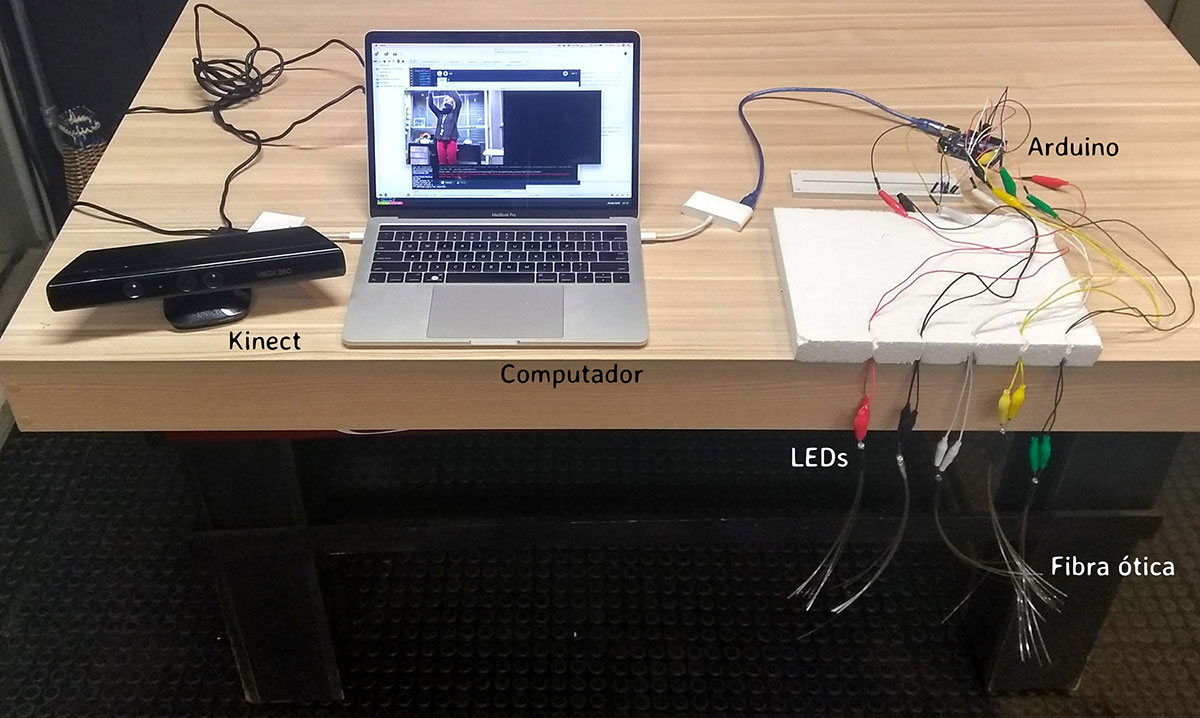
\includegraphics[width=0.8\textwidth]{./04-figuras/prototipo}
    \label{fig:prototipo}
\end{figure}
\vspace*{-0,9cm}
{\raggedright \fonte{Elaborada pela autora}}\\

Na figura \ref{fig:prototipo-escuro} podemos ver uma amostra do protótipo sendo executado em um ambiente com baixa luminosidade. Constatou-se que a luz conseguia se propagar ao longo da fibra, mas que se mostrava com maior intensidade em suas extremidades. A partir disso pensou-se na proposta de junção dos LEDs com a fibra ótica apresentada na seção \ref{sec:malha} deste capítulo.
 
\begin{figure}[H]
    \centering
    \caption{Protótipo em ambiente com baixa luminosidade}
	\vspace*{0,2cm}
    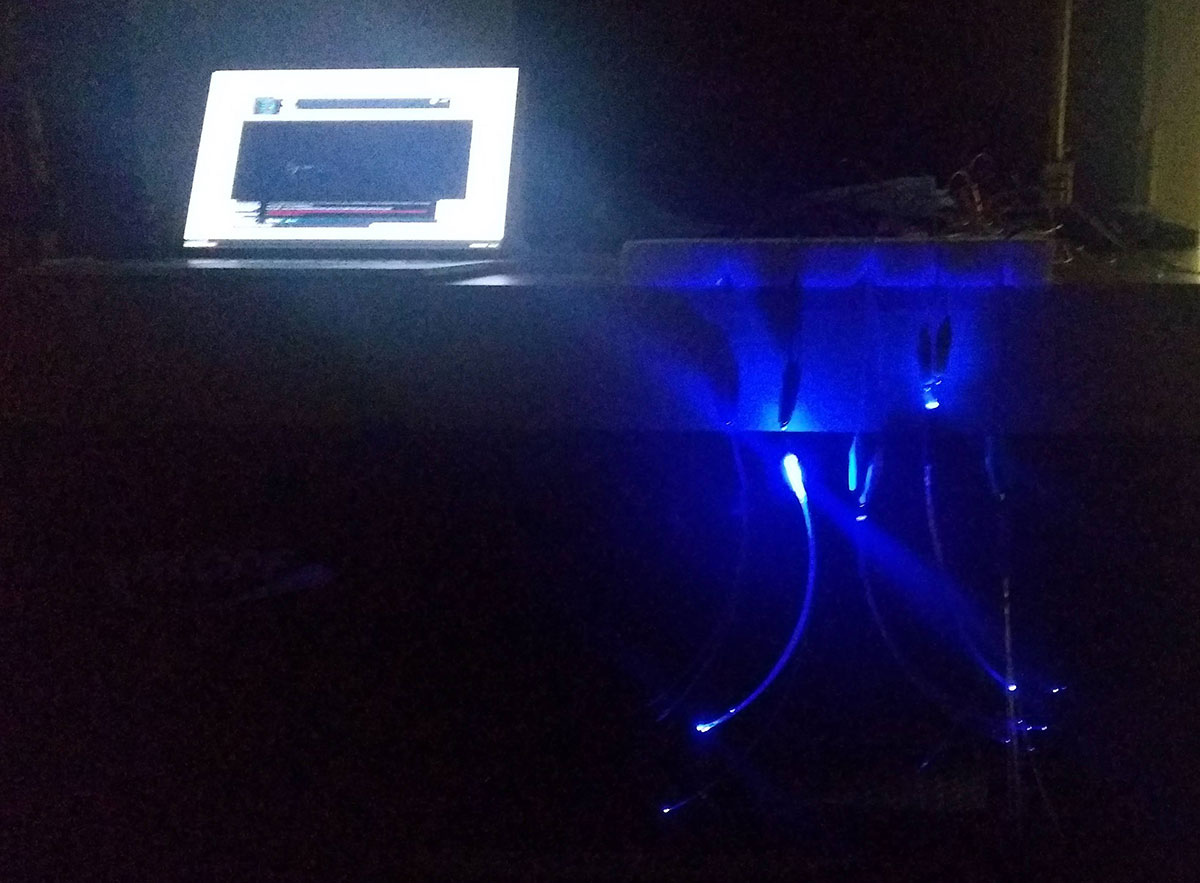
\includegraphics[width=0.8\textwidth]{./04-figuras/prototipo_escuro}
    \label{fig:prototipo-escuro}
\end{figure}
\vspace*{-0,9cm}
{\raggedright \fonte{Elaborada pela autora}}\\

No que diz respeito a integração dos elementos presentes na obra, foi possível constatar seu correto funcionamento já em conformidade com o modelo da proposta introduzida no início deste capítulo, pois os dispositivos utilizados aqui eram os mesmos ou muito similares aos que encontramos no trabalho final. A partir disso, o desafio se concentrou em construir a malha de LEDs, bem como fazer a colagem da fibra ótica em cada um deles, além de criar a versão final do \textit{script} que deveria funcionar como uma matriz e carecia de uma otimização em sua lógica de detecção de presença.

   